\section{Les Frappes de Processus standards}
\seclabel{ph}

Cette section définit les Frappes de Processus standards
telles qu'elles ont été formalisées par \citeasnoun{PMR10-TCSB}.
En tant que restrictions du $\pi$\nbd calcul \cite{Brand83,Milner89},
les Frappes de Processus offrent une représentation discrète, asynchrone et indéterministe
avec une définition atomique des interactions entre les différents composants du modèle.
En cela,
elles sont particulièrement adaptées aux représentations des réseaux de régulation biologique
bien qu'elles soient assez générales pour potentiellement permettre des applications plus
larges en informatique ou dans d'autres domaines.

Nous donnerons tout d'abord à la \secref{ph} une définition des Frappes de Processus standards
%accompagnée d'une discussion,
ainsi qu'un certain nombre de définitions formelles supplémentaires
nécessaires pour la suite de ce manuscrit.
Nous détaillons ensuite à la \secref{sc} le mécanisme particulier des sortes coopératives
tel qu'il avait été formalisé dans les travaux de Loïc Paulevé,
et nous montrerons qu'il permet de représenter l'action conjointe de plusieurs composants,
mais avec certains défauts difficiles à corriger dans cette version du formalisme.
Enfin, nous aborderons brièvement les travaux précédents
concernant l'analyse statique qui permet d'obtenir des résultats
sur l'ensemble des états stables (\secref{ph-pf})
et sur l'atteignabilité d'un niveau local au sein d'un modèle (\secref{ph-as}),
et nous évoquerons les possibilités d'ajout de paramètres stochastiques (\secref{ph-stocha})
dans le but d'introduire une composante temporelle continue dans les Frappes de Processus.



\subsection{Définition des Frappes de Processus standards}
\seclabel{ph-def}

Les \emph{Frappes de Processus standards} telles que données à la \defref{ph},
aussi appelées \textit{Process Hitting},
ou plus simplement \emph{Frappes de Processus} dans ce chapitre,
permettent une modélisation atomique et asynchrone des interactions entre composants.
Un modèle de Frappes de Processus standards comporte un nombre fini de \emph{sortes}
généralement notées $a$, $b$, $c$...
Celles-ci permettent de représenter les différentes entités du modèle,
qu'il s'agisse de composant ayant une réalité biologique (gène, protéine...)
ou d'entités nécessaire à la modélisation (comme les sortes coopératives
qui seront décrites à la \secref{sc}).
Chaque sortes contient plusieurs \emph{processus},
qui représentent les différents
niveaux d'expression discrets accessibles par la sorte,
et qui sont notés $a_i$
où $a$ est le nom de la sorte et $i$ l'indice du processus dans cette sorte.
Un processus n'appartient qu'à une unique sorte.
Chaque processus est dit \emph{actif} s'il représente le niveau d'expression
dans lequel doit se trouver sa sorte à un certain moment.
Un \emph{état} du modèle est donc décrit par l'ensemble des processus actifs à un instant donné,
avec exactement un processus actif par sorte
---~afin de ne pas sur-représenter ou sous-représenter le niveau d'expression courant d'une sorte.

La dynamique est introduite dans les Frappes de Processus par des \emph{actions}
qui permettent de modifier le processus actif d'une sorte,
à la condition éventuelle qu'un processus donné d'une autre sorte soit présent.
Une action consiste donc en un triplet de processus $\PHfrappe{a_i}{b_j}{b_k}$
qui se lit : «~$a_i$ frappe $b_j$ pour le faire bondir en $b_k$~»,
et qui signifie que si, dans un état donné, les processus $a_i$ et $b_j$ sont
tous les deux présents, alors il est possible d'activer $b_k$ (et de désactiver $b_j$)
dans l'état suivant.
Autrement dit, le processus actif de la sorte $b$ peut \emph{bondir}
de $b_j$ à $b_k$ à condition que $a_i$ soit actif ;
lorsque cela arrive, on dit qu'on a \emph{joué} l'action $\PHfrappe{a_i}{b_j}{b_k}$.
Par convention, on contraint de plus que $b_j \neq b_k$ pour assurer que le jeu d'une action
provoque bien un changement de processus actif.
Il est aussi possible de définir une auto-action, où $a_i = b_j$ (et nécessairement $a = b$),
qui permet de représenter le cas particulier où le processus $b_j$ peut bondir en $b_k$
sans autre condition.

Les Frappes de Processus sont conçues comme un formalisme
à temps discret asynchrone, ce qui signifie que
l'évolution d'un tel modèle est modélisée par une succession de pas de temps discrets
qui représentent la succession des états du modèle,
et exactement une action est jouée entre deux états successifs.
Cela implique qu'un seul processus actif à la fois peut bondir entre deux
pas de temps successifs, et donc qu'une seule sorte peut évoluer entre deux états.
De plus, cela rend la dynamique Frappes de Processus indéterministe,
car à tout état du modèle peuvent correspondre plusieurs états successeurs
dans le cas où plusieurs actions peuvent y être jouées.
Enfin, nous notons que si aucune action n'est jouable dans un état, alors celui-ci
ne possède pas de successeur et le modèle ne peut plus évoluer.

\begin{definition}[Frappes de Processus standards]
\deflabel{ph}
  Les \emph{Frappes de Processus standards} sont définies
  par un triplet $\PH = (\PHs; \PHl; \PHh)$, où :
  \begin{itemize}
    \item $\PHs \DEF \{a, b, \dots\}$ est l'ensemble fini et dénombrable des \emph{sortes} ;
    \item $\PHl \DEF \bigtimes{a \in \PHs} \PHl_a$ est l'ensemble fini des \emph{états},
      où $\PHl_a = \{a_0, \ldots, a_{l_a}\}$ est l'ensemble fini et dénombrable
      des \emph{processus} de la sorte $a \in \PHs$ et $l_a \in \sN^*$,
      chaque processus appartenant à une unique sorte :
      $\forall (a_i; b_j) \in \PHl_a \times \PHl_b, a \neq b \Rightarrow a_i \neq b_j$ ;
    \item $\PHh \DEF \{\PHfrappe{a_i}{b_j}{b_k} \mid (a; b) \in \PHs \times \PHs \wedge
      (a_i; b_j; b_k) \in \PHl_a \times \PHl_b \times \PHl_b \wedge
      b_j \neq b_k \wedge a = b \Rightarrow a_i = b_j \}$ est l'ensemble fini des \emph{actions}.
  \end{itemize}
\end{definition}
%
\noindent
On note $\PHproc \DEF \bigcup_{a \in \PHs} \PHl_a$ l'ensemble de tous les processus.
La sorte d'un processus $a_i$ est donnée par $\PHsort(a_i) = a$ ;
on définit aussi l'ensemble des sortes d'une action ou d'un ensemble de processus par :
\begin{align*}
  \forall h \in \PHh, \sortes{h} &= \{ \sorte{\frappeur{h}}, \sorte{\cible{h}} \} \\
  \forall A \subset \Proc, \sortes{A} &= \{ \sorte{p} \mid p \in A \}
\end{align*}
Étant donné un état $s \in \PHl$, le processus de la sorte $a \in \PHs$ présent dans $s$ est donné
par $\PHget{s}{a}$, \cad la coordonnée correspondant à $a$ dans l'état $s$.
Si $a_i \in \PHl_a$, nous définissons la notation : $a_i \in s \EQDEF \PHget{s}{a} = a_i$ ;
par extension, si $ps \subset \Proc$, on écrit alors :
$ps \subseteq s \EQDEF \forall p \in ps, p \in s$.
Pour toute action $h = \PHfrappe{a_i}{b_j}{b_k} \in \PHh$,
$a_i$ est appelé le \emph{frappeur}, $b_j$ la \emph{cible} et $b_k$ le \emph{bond} de $h$,
et on note : $\hitter{h} = a_i$, $\target{h} = b_j$ et $\bounce{h} = b_k$.

\begin{example}
\exlabel{metazoan-ph-nocoop}
  La \figref{metazoan-ph-nocoop} illustre une représentation possible des
  Frappes de Processus standards.
  Le modèle $\PH = (\PHs, \PHl, \PHh)$ représenté comporte trois sortes :
  $\PHs = \{ a, c, f \}$.
  Chaque sorte comporte exactement deux processus :
  \[\PHl_a = \{ a_0, a_1 \} \enspace;\quad
    \PHl_b = \{ b_0, b_1 \} \enspace;\quad
    \PHl_f = \{ f_0, f_1 \} \enspace.\]
  On peut notamment en déduire le nombre total d'états du système :
  $\card{\PHl} = 2^3 = 8$.
  Enfin, ce modèle comporte 7 actions :
  \begin{align*}
    \PHh = \{\qquad
      \PHfrappe{c_1}{a_1}{a_0}\quad, && \PHfrappe{c_0}{a_0}{a_1}\quad,& \\
      \PHfrappe{c_1}{c_1}{c_0}\quad, && \PHfrappe{f_1}{c_0}{c_1}\quad,& \\
      \PHfrappe{f_1}{a_0}{a_1}\quad, && \PHfrappe{f_0}{c_1}{c_0}\quad,& \\
      \PHfrappe{f_1}{f_1}{f_0}\quad\; &&& 
    \qquad\}
  \end{align*}
  
  Ces Frappes de Processus représentent un modèle simplifié du mécanisme
  de segmentation des métazoaires qui permet par exemple de décrire la production de rayures
  chez les drosophiles.
  Il a été originellement établi \textit{in silico} par \citeasnoun{MSB4100192}
  à l'aide d'un formalisme à base d'équations différentielles,
  et le modèle présenté ici est inspiré du modèle proposé par \citeasnoun{PMR10-TCSB}.
  
  Les trois sortes $a$, $b$ et $c$ de ce modèle représentent différents gènes du système,
  que nous qualifierons d'\emph{actifs} dans le reste de ce document lorsqu'ils seront à l'état 1.
  La production de pigment est déclenchée par le produit du gène $a$,
  et une succession d'activations de celui-ci permet donc de produire des rayures.
  Pour que celles-ci soient régulières, il est donc nécessaire que la durée d'activation
  de $a$ soit constante, et que la durée entre deux activations le soit aussi.
  Ce mécanisme est réglé par le gène $c$ qui inhibe à la fois le gène $a$ à intervalles réguliers,
  et s'inhibe lui-même afin d'avoir le rôle d'une horloge.
  Enfin, le procédé complet est dirigé par le gène $f$ qui, lorsqu'il est actif,
  permet la progression d'un front au niveau duquel les pigments sont déposés.
  Ce gène peut aussi s'auto-inhiber après une certaine période, faisant cesser
  l'oscillation de l'horloge et ainsi la production de rayures.
  
  \begin{figure}[ht]
  \begin{center}
  \scalebox{1.5}{\begin{tikzpicture}
    \TSort{(0,4)}{c}{2}{l}
    \TSort{(1,1)}{f}{2}{l}
    \TSort{(3,4)}{a}{2}{r}
    
    \TAction{c_1}{a_1.west}{a_0.north west}{}{right}
    \TAction{f_1}{c_0.west}{c_1.south west}{bend left=50, in=90}{left}
    \TAction{c_1}{c_1.west}{c_0.north west}{selfhit}{right}
    \TAction{f_1.north east}{f_1.south east}{f_0.north east}%
      {selfhit, min distance=30, bend left, out=150, in=90}{left}
    \TAction{f_0.east}{c_1.south east}{c_0.north east}{bend right=80, in=-120}{left}
    
    % Fausse coopération
    \TAction{f_1.north}{a_0.south west}{a_1.south west}{bend left=20}{left}
    \TAction{c_0}{a_0.west}{a_1.south}{}{left}
    
    \TState{f_1, a_0, c_0}
  \end{tikzpicture}}
  \caption{\figlabel{metazoan-ph-nocoop}%
    Un exemple de Frappes de Processus standards.
    Les sortes sont représentées par des rectangles arrondis 
    contenant des cercles représentant les processus.
    Ainsi, le processus $a_1$ est représenté par le cercle marqué «~1~»
    dans le rectangle étiqueté «~$a$~», etc.
    Chaque action est de plus symbolisée par un couple de flèches,
    l'une en trait plein et l'autre en pointillés ;
    par exemple, l'action $\PHfrappe{c_1}{a_1}{a_0}$
    est représentée par une flèche pleine entre les processus $c_1$ et $a_1$
    suivie d'une flèche en pointillés entre $a_1$ et $a_0$.
    Enfin, les processus grisés représentent un état possible
    pour ces Frappes de Processus : $\etat{a_0, c_0, f_1}$, qui peut aussi faire office
    d'état initial pour ce modèle.
  }
  \end{center}
  \end{figure}
\end{example}

Les séquences d'actions ont un rôle particulier pour les Frappes de Processus.
Elles permettent notamment d'abstraire une dynamique locale en se concentrant
sur la conséquence plutôt que sur la cause,
et seront notamment utiles pour la méthode d'analyse statique développée
au \chapref{phcanonique}.
Pour toute séquence d'actions $A$,
on note $\sortes{A}$ l'ensemble des sortes dont au moins un processus figure dans $A$
en tant que frappeur, cible ou bond d'une action.
De plus, pour toute sorte $a$,
on note $\prem{a}{A}$ le premier processus de $a$ référencé dans $A$,
en tant que frappeur ou en tant que cible,
et $\der{a}{A}$ le dernier, en tant que frappeur ou en tant que bond.
On note en conséquence
$\sup{A}$ l'ensemble de tous ces premiers processus,
et $\fin{A}$ l'ensemble de tous ces derniers processus.

\begin{definition}[$\premsymbol$, $\dersymbol$, $\suppsymbol$ et $\finsymbol$]
\deflabel{premder}
%   Pour toute séquence d'actions $A$ et pour toute sorte $a$,
%   $\prem{a}{A}$ est le premier processus de $a$ référencé dans $A$,
%   en tant que frappeur ou en tant que cible,
%   et $\der{a}{A}$ en est le dernier,
%   en tant que frappeur ou en tant que bond.
  \begin{align*}
%   \eqlabel{prem}
    \prem{a}{A} &=
      \begin{cases}
        \varnothing & \text{si } a \notin \sortes{A} \\
        \hitter{A_m} & \text{si } m = \min\{ n \in \indexes{A} \mid a \in \sortes{A_n} \}
          \wedge \sorte{\hitter{A_m}} = a \\
        \target{A_m} & \text{sinon si } m = \min\{ n \in \indexes{A} \mid a \in \sortes{A_n} \}
          \wedge \sorte{\target{A_m}} = a
      \end{cases} \\
%   \eqlabel{der}
    \der{a}{A} &=
      \begin{cases}
        \varnothing & \text{si } a \notin \sortes{A} \\
        \bounce{A_m} & \text{si } m = \max\{ n \in \indexes{A} \mid a \in \sortes{A_n} \}
          \wedge \sorte{\bounce{A_m}} = a \\
        \hitter{A_m} & \text{sinon si } m = \max\{ n \in \indexes{A} \mid a \in \sortes{A_n} \}
          \wedge \sorte{\hitter{A_m}} = a
      \end{cases}
  \end{align*}
%   Pour toute séquence d'actions $A$,
%   $\supp{A}$ et $\fin{A}$ renvoient respectivement à l'ensemble des premiers
%   et derniers processus de $A$ pour toutes les sortes qui y figurent.
  \begin{align*}
%   \eqlabel{supp}
    \supp{A} &= \{ p \in \Proc \mid \sorte{p} \in \sortes{A} \wedge
      p = \prem{\sort{p}}{\delta} \} \\
%   \eqlabel{fin}
    \fin{A} &= \{ p \in \Proc \mid \sorte{p} \in \sortes{A} \wedge
      p = \der{\sort{p}}{\delta} \}
  \end{align*}
\end{definition}

La \defref{substate} établit la notion de sous-état sur un ensemble de sortes,
\cad un ensemble de processus qui sont deux à deux de sortes différentes,
ce qui permet de ne considérer qu'une partie d'un état complet.
Nous notons $\PHsubl$ l'ensemble de tous les sous-états et nous constatons qu'un
état est \textit{a fortiori} un sous-état : $\PHl \subset \PHsubl$.
Nous notons de plus $\PHsublset$ l'ensemble des sous-états désordonnés,
c'est-à-dire dont l'ordre entre les sortes a été oublié.
Le recouvrement d'un état $s$ par un processus $a_i$ est formalisé à la \defref{recouvrement}
par un état identique à $s$, sauf pour le processus de $a$ qui a été remplacé par $a_i$,
ce qui permettra de définir la dynamique des Frappes de Processus %avec $k$ classes de priorités
à la \defref{play}.
La définition de recouvrement est aussi étendue à un sous-état désordonné,
autrement dit, à un ensemble de processus contenant au plus un processus par sorte.

\begin{definition}[Sous-états ($\PHsublize{\PHl}$)]
\deflabel{substate}
  Si $S \subset \PHs$ est un ensemble de sortes, un sous-état sur $S$ est un élément de :
  $\PHsubl[\PHl]_S \DEF \bigtimes{a \in S} \PHl_a$.
  L'ensemble de tous les sous-états est noté :
  $\PHsubl[\PHl] \DEF \bigcup_{S \in\powerset(\PHs)} \PHsubl[\PHl]_S$.
  
  \noindent
  De plus, si $\mysigma \in \PHsubl[\PHl]$ et $s \in \PHl$, on note alors :
  \[\mysigma \subseteq s \EQDEF \forall a_i \in \Proc, a_i \in \mysigma \Rightarrow a_i \in s
    \enspace.\]
  
  \noindent
  Enfin, si $S \subset \PHs$, on note :
  $\PHsublset_S = \{ \toset{ps} \subset \Proc \mid ps \in \PHsubl_S \}$
  et
  $\PHsublset = \{ \toset{ps} \subset \Proc \mid ps \in \PHsubl \}$.
\end{definition}
%
\begin{definition}[Recouvrement ($\recouvre : \PHl \times \PHproc \rightarrow \PHl$)]
\deflabel{recouvrement}
  Étant donné un état $s \in \PHl$ et un processus $a_i \in \PHproc$,
  $(s \recouvre a_i)$ est l'état défini par :
  $\PHget{(s \recouvre a_i)}{a} = a_i \wedge
    \forall b \neq a, \PHget{(s \recouvre a_i)}{b} = \PHget{s}{b}$.
  On étend de plus cette définition à un ensemble de processus
  par le recouvrement de l'état par chaque processus,
  à condition que les processus de l'ensemble soient tous de sortes différentes :
  $\forall ps \in \PHsublset, s \recouvre ps = s \underset{a_i \in ps}{\recouvre} a_i$.
\end{definition}

Nous définissons dans la suite les outils nécessaires à la dynamique des Frappes de Processus.
Pour cela, nous introduisons la notion de propriété de jouabilité à la \defref{ppl},
qui est semblable à une formule booléenne dont les atomes sont des processus dans $\Proc$.
Le langage des propriétés de jouabilité permet de décrire la présence d'une configuration
de processus actifs dans un état donné, ce qui
permet donc notamment de décrire en termes formels la jouabilité d'une action.
Cela est mis en pratique pour les Frappes de Processus standards à la \defref{fopph}
où nous définissons l'\emph{opérateur de jouabilité} de ce formalisme,
qui est une formule associant à chaque action sa propriété de jouabilité propre.
Pour finir, la dynamique des Frappes de Processus est donnée à la \defref{play}
à partir de celle d'opérateur de jouabilité.
Les définitions de propriété de jouabilité (\defref{ppl}) et de dynamique des Frappes de Processus
(\defref{play}) sont volontairement assez générales pour pouvoir être réutilisées au
\chapref{sem} pour définir la sémantique d'autres formalismes de Frappes de Processus.

\begin{definition}[Propriété de jouabilité ($\F$)]
\deflabel{ppl}
  Une \emph{propriété de jouabilité} est un élément du langage $\F$ défini inductivement par :
  \begin{itemize}
    \item $\top$ et $\bot$ appartiennent à $\F$ ;
    \item si $a \in \PHs$ et $a_i \in \PHl_a$, alors $a_i$ appartient à $\F$
      et est appelé un \emph{atome} ;
    \item si $P \in \F$ et $Q \in \F$,
      alors $\neg P$, $P \wedge Q$ et $P \vee Q$ appartiennent à $\F$.
  \end{itemize}
%
  Si $P \in \F$ est une propriété de jouabilité et $\mysigma \in \PHsubl$ est un sous-état,
  on note $\Feval{P}{\mysigma}$ l'\emph{évaluation} de $P$ dans $\mysigma$:
  \begin{itemize}
    \item si $P = a_i \in \PHl_a$ est un atome, avec $a \in \PHs$,
      alors $\Feval{a_i}{\mysigma}$ est vraie si et seulement si $a_i \in \mysigma$ ;
    \item si $P$ n'est pas un atome, alors $\Feval{P}{\mysigma}$ est vraie si et seulement si
      on peut l'évaluer récursivement comme vraie en utilisant la sémantique habituelle des
      opérateurs $\neg$, $\wedge$ et $\vee$ et des constantes $\top$ et $\bot$.
  \end{itemize}
%
  Une fonction $\Fopsymbol : \PHh \rightarrow \F$ associant à toute action une propriété de jouabilité
  est appelée un \emph{opérateur de jouabilité}.
\end{definition}

Étant donné que ce langage n'utilise que des opérateur logiques classiques,
les propriétés de la logique booléenne sont applicables aux propriétés de jouabilité,
à savoir celles concernant la distributivité, l'associativité et la commutativité,
ainsi que les lois de De Morgan concernant la négation.

Il en résulte notamment la propriété suivante, permettant d'évaluer la négation d'un atome,
et qui dérive naturellement du fait que si un processus n'est pas actif dans un état donné,
cela signifie alors qu'un autre processus de la même sorte l'est :
\[\forall a \in \PHs, \forall a_i \in \PHl_a, \forall \mysigma \in \PHsubl,
  \Feval{\neg a_i}{\mysigma} \Leftrightarrow
  \Feval{\bigvee_{\substack{a_j \in \PHl_a\\a_j \neq a_i}} a_j}{\mysigma}\]

% Enfin, on note dans la suite :
% \[\forall A \in \PHsublset, \Fconj{A} \equiv \bigwedge_{p \in A} p \enspace.\]

L'opérateur de jouabilité $\Fopsymbol$ donné à la \defref{fopph} est propre aux
Frappes de Processus standards.
En revanche, la dynamique donnée à la \defref{play} est générale à toutes les
Frappes de Processus, et peut donc à fortiori être utilisée avec l'opérateur $\Fopsymbol$
des Frappes de Processus standards.

\begin{definition}[Opérateur de jouabilité ($\Fopsymbol : \PHh \rightarrow \F$)]
\deflabel{fopph}
  L'opérateur de jouabilité des Frappes de Processus est défini par :
  \[\forall h \in \PHh, \Fop{h} \equiv \hitter{h} \wedge \target{h} \enspace.\]
\end{definition}

\begin{definition}[Dynamique des Frappes de Processus ($\PHtrans$)]
\deflabel{play}
  Une action $h \in \PHh$ est dite \emph{jouable}
  dans l'état $s \in \PHl$ si et seulement si :
  $\Feval{\Fop{h}}{s}$.
%  $\target{h} \in s \wedge \Feval{\Fop{h}}{s}$.
  Dans ce cas, $(s \PHplay h)$ est l'état résultant du jeu de l'action $h$ dans $s$,
  et on le définit par : $(s \PHplay h) = s \recouvre \bounce{h}$.
  De plus, on note alors : $s \PHtrans (s \PHplay h)$.

  Si $s \in \PHl$, un \emph{scénario} $\delta$ dans $s$
  est une séquence d'actions de $\PHh$ qui peuvent être jouées successivement dans $s$.
  L'ensemble de tous les scénarios dans $s$ est noté $\Sce(s)$.
\end{definition}



\begin{remark}
  Les Frappes de Processus standards possèdent une dynamique totalement asynchrone :
  entre deux états, une unique action peut être jouée.
  Ce choix de conception est largement inspiré du modèle de Thomas
  présenté à la \vsecref{thomas-def},
  dont la dynamique est aussi totalement asynchrone.
  Biologiquement, une telle hypothèse est cohérent avec le fait que la probabilité
  que deux composants franchissent simultanément un seuil d'expression est très faible.
  Cependant, cette sémantique asynchrone permet aussi de simplifier la dynamique des
  Frappes de Processus standards en assurant que deux états successifs ne varient
  que d'un seul processus (en fait : exactement d'un processus).
  Cela a notamment permis le développement de l'analyse statique évoquée
  plus loin, à la \secref{ph-as}.
\end{remark}



\begin{example}
  La dynamique des Frappes de Processus standards de la \figref{metazoan-ph-nocoop}
  est représentée à la \figref{metazoan-nocoop-dynamique}.
  On peut notamment y observer le comportement stationnaire normal du modèle
  qui consiste en une oscillation alternée des processus actifs des sortes $a$ et $c$ :
%  où on a représenté en gras le processus modifié par rapport à l'état précédent :
  \[\etat{a_0,c_0,f_1} \PHtrans \etat{a_1,c_0,f_1}
    \PHtrans \etat{a_1,c_1,f_1} \PHtrans \etat{a_0,c_1,f_1}
    \PHtrans \etat{a_0,c_0,f_1} \PHtrans \ldots\]
  
  \begin{figure}[ht]
    \begin{center}
    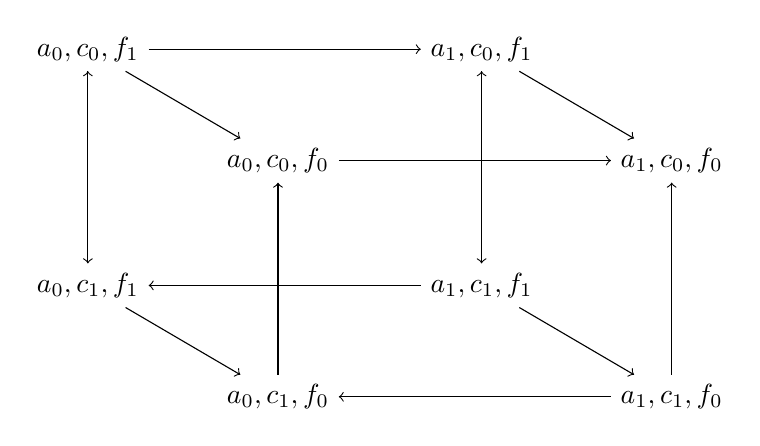
\begin{tikzpicture}[node distance=3cm]
      \node (s001) {$\etat{a_0,c_0,f_1}$};
      \node[below of=s001] (s011) {$\etat{a_0,c_1,f_1}$};
      \node[right of=s001, node distance=5cm] (s101) {$\etat{a_1,c_0,f_1}$};
      \node[below of=s101] (s111) {$\etat{a_1,c_1,f_1}$};
      \node[below right of=s001, node distance=2cm, xshift=1cm] (s000) {$\etat{a_0,c_0,f_0}$};
      \node[below of=s000] (s010) {$\etat{a_0,c_1,f_0}$};
      \node[right of=s000, node distance=5cm] (s100) {$\etat{a_1,c_0,f_0}$};
      \node[below of=s100] (s110) {$\etat{a_1,c_1,f_0}$};
      
      \path[->]
        (s001) edge (s000) edge (s101)
        (s011) edge (s010)
        %
        (s001) edge (s011)
        (s011) edge (s001)
        %
        (s101) edge (s100) edge (s111)
        (s111) edge (s101) edge (s110) edge (s011)
        (s000) edge (s100)
        (s010) edge (s000)
        (s110) edge (s100) edge (s010)
      ;
    \end{tikzpicture}
    \end{center}
    \caption{\figlabel{metazoan-nocoop-dynamique}%
      Représentation de la dynamique du modèle de Frappes de Processus standards
      de la \figref{metazoan-ph-nocoop}.
      Chaque état est représenté par un triplet $\etat{a_i, c_j, f_k}$
      où $i$, $j$ et $k$ représentent respectivement le niveau d'expression de $a$, $c$ et $f$.
      Une transition entre deux états est représentée par une flèche.
    }
  \end{figure}
\end{example}



\subsection{Utilisation des sortes coopératives}
\seclabel{sc}

L'une des questions qui se posent face à un formalisme totalement asynchrone comme
les Frappes de Processus standards est la représentation des coopérations entre les différents
composants.
En effet, le bond d'un processus dans un modèle de Frappes de Processus standards
ne peut se faire que par le jeu d'une action,
elle-même déclenchée par la présence d'au plus deux processus :
le frappeur et la cible (c'est-à-dire le processus qui va bondir).
Il n'est donc pas possible de conditionner le bond d'un processus par la présence
de plusieurs processus de sortes différentes de celle de la cible.
En effet,
si on souhaite par exemple représenter l'activation d'un processus $c_1$ (d'une sorte $c$)
uniquement lorsque deux autres processus $a_1$ et $b_1$ (de deux autres sortes $a$ et $b$)
sont actifs, il n'est pas suffisant d'ajouter deux actions
$\PHfrappe{a_1}{c_0}{c_1}$ et $\PHfrappe{b_1}{c_0}{c_1}$,
car celles-ci permettent d'activer $c_1$ à la condition que $a_1$ ou $b_1$
soit présent : il s'agit bien de deux interactions distinctes et non d'une coopération.

\begin{example}
\exlabel{metazoan-ph-nocoop-explications}
  Le modèle de Frappes de Processus de la \figref{metazoan-ph-nocoop}
  représente le mécanisme de segmentation métazoaire évoqué à la page
  \expageref{metazoan-ph-nocoop}.
  Dans ce modèle, la production de pigment devrait uniquement être possible
  à la condition suivante : «~$f$ est actif et $c$ n'est pas actif~».
  Or dans l'état courant du modèle,
  la désactivation du gène $f$ n'empêche pas la production de pigment,
  car depuis tout état contenant $f_0$, il est toujours possible d'activer $a$
  à l'aide des actions $\PHfrappe{f_0}{c_1}{c_0}$ et $\PHfrappe{c_0}{a_0}{a_1}$.
\end{example}

Afin de représenter la coopération entre composants,
et donc le raffinement de la dynamique des modèles,
\citeasnoun{PMR10-TCSB} ont proposé d'ajouter des sortes particulières appelées
\emph{sortes coopératives}, qui servent exclusivement à la modélisation.
Une sorte coopérative permet de représenter l'état conjoint de plusieurs sortes dans le modèle.
Pour cela, à chaque processus de la sorte coopérative correspond un sous-état des sortes
qu'elle \emph{représente}.
Ainsi, il est possible de représenter les différents états combinés d'un ensemble de sortes,
afin de ne jouer une action que dans une configuration particulière.
Ces sortes ont l'avantage d'être des sortes standards,
et donc de ne pas nécessiter d'enrichissement particulier de la sémantique.
De plus, leur utilisation n'impacte pas les méthodes d'analyse de la dynamique développées :
en effet, ces méthodes sont principalement impactées par le nombre de processus dans chaque sorte,
et non le nombre total de sortes.
Ainsi, à condition de limiter le nombre de processus dans les sortes coopératives,
comme expliqué à la fin de cette section,
il est possible de les utiliser en maintenant de bonnes performances d'analyse.

\begin{example}
  Les Frappes de Processus standards de la \figref{excoop-ph}
  reprennent les trois sortes $f$, $c$ et $a$ du modèle de la \figref{metazoan-ph-nocoop}
  et comprennent en plus une sorte coopérative $fc$
  permettant de détecter la présence simultanée de $f_1$ et $c_1$.
  Les processus de $fc$ décrivent les combinaisons possibles des états de $f$ et de $c$ :
  $fc_{00}$ correspond à $f_0$ et $c_0$, $fc_{01}$ correspond à $f_0$ et $c_1$, etc.
  Les actions en amont de cette sorte coopérative permettent la mettre à jour,
  c'est-à-dire de changer son processus actif en fonction des évolutions
  du processus actif de $f$ et $c$.
  Par exemple, si $f_1$ est actif, les deux actions
  $\PHfrappe{f_1}{fc_{00}}{fc_{10}}$ et $\PHfrappe{f_1}{fc_{01}}{fc_{11}}$
  effectuent cette mise à jour en faisant bondir le processus actif de $fc$ depuis
  un processus représentant la présence de $f_0$ ($fc_{00}$ ou $fc_{01}$)
  vers le processus correspondant représentant la présence de $f_1$
  (respectivement $fc_{10}$ ou $fc_{11}$).
  Son action en aval, $\PHfrappe{fc_{11}}{c_0}{c_1}$,
  joue alors le rôle d'une coopération entre $f_1$ et $c_0$
  pour frapper $a_0$ et le faire bondir en $a_1$.
  
  \begin{figure}[p]
  \begin{center}\scalebox{1.2}{
  \begin{tikzpicture}
    \TSort{(0,0)}{f}{2}{l}
    \TSort{(0,4)}{c}{2}{l}
    \TSort{(7,2)}{a}{2}{r}

    \TSetTick{fc}{0}{00}
    \TSetTick{fc}{1}{01}
    \TSetTick{fc}{2}{10}
    \TSetTick{fc}{3}{11}
    \TSort{(4,1)}{fc}{4}{r}

    \THit{f_0}{}{fc_3}{.west}{fc_1}
    \THit{f_0}{}{fc_2}{.south west}{fc_0}
    \THit{f_1}{}{fc_1}{.west}{fc_3}
    \THit{f_1}{}{fc_0}{.south west}{fc_2}

    \THit{c_0}{}{fc_3}{.north west}{fc_2}
    \THit{c_0}{}{fc_1}{.north west}{fc_0}
    \THit{c_1}{}{fc_2}{.west}{fc_3}
    \THit{c_1}{}{fc_0}{.west}{fc_1}

    \THit{fc_2}{}{a_0}{.west}{a_1}

    \path[bounce, bend right = 70]
      \TBounce{fc_3}{}{fc_1}{.north}
      \TBounce{fc_2}{}{fc_0}{.north west}
      \TBounce{fc_3}{}{fc_2}{.north west}
      \TBounce{fc_1}{}{fc_0}{.north}
    ;
    \path[bounce, bend left = 70]
      \TBounce{fc_1}{}{fc_3}{.south}
      \TBounce{fc_0}{}{fc_2}{.south}
      \TBounce{fc_2}{}{fc_3}{.south west}
      \TBounce{fc_0}{}{fc_1}{.south west}
    ;
    \path[bounce, bend left]
      \TBounce{a_0}{}{a_1}{.south west}
    ;
    %\TState{a_0, b_0, ab_0, c_0}
  \end{tikzpicture}
  }\end{center}
  \caption{\figlabel{excoop-ph}%
    Un exemple de Frappes de Processus standards
    avec une sorte coopérative $fc$.
    L'action $\PHfrappe{fc_{10}}{a_0}{a_1}$ modélise
    une coopération entre $f_1$ et $c_0$ pour faire bondir le processus actif de $a$.}
  \end{figure}
\end{example}

\begin{example}
\exlabel{metazoan-ph}
  Afin de pallier partiellement l'absence de coopération entre les sortes $f$ et $c$
  dans le modèle de la \figref{metazoan-ph-nocoop},
  il est possible d'intégrer la sorte coopérative
  décrite à la \figref{excoop-ph}.
  La \figref{metazoan-ph} propose un modèle corrigé de cette manière,
  avec une sorte coopérative $fc$ permettant de détecter la présence de $f_1$ et $c_0$.
  Les deux actions $\PHfrappe{c_0}{a_0}{a_1}$ et $\PHfrappe{c_0}{a_0}{a_1}$
  sont alors remplacées par une action $\PHfrappe{fc_{10}}{a_0}{a_1}$
  afin d'avoir une véritable coopération entre ces deux processus pour activer $a$.
  
  \begin{figure}[p]
  \begin{center}
  \begin{tikzpicture}
    \exmetazoan
    
    \TState{f_1, a_0, c_0, fc_2}
  \end{tikzpicture}
  \caption{\figlabel{metazoan-ph}%
    Amélioration du modèle de Frappes de Processus de la \figref{metazoan-ph-nocoop}
    à l'aide de la sorte coopérative $fc$.
    Les processus de cette sorte représentent les différents sous-états formés par les
    deux sortes $f$ et $c$.
    Ainsi, $fc_{00}$ représente le fait que $f_0$ et $c_0$ sont actifs, etc.
    Les actions permettant la mise à jour de cette sorte coopérative n'ont pas
    été représentées explicitement mais sont symbolisées par les deux flèches
    en zigzag provenant de $f$ et $c$.
  }
  \end{center}
  \end{figure}
\end{example}

\myskip

Le sortes coopératives possèdent cependant un défaut, qui est lié au fait que les actions
sont totalement indépendantes, car
le formalisme des Frappes de Processus standards est totalement asynchrone et indéterministe.
En effet, les sortes coopératives ne sont pas nécessairement mises à jour immédiatement
après un bond du processus actif d'une des sortes qu'elles représentent.
Il peut ainsi exister un «~décalage temporel~» entre le changement de processus actif
d'une sorte et la mise à jour des sortes coopératives.
%Ce décalage temporel introduit des comportements indésirables sur deux niveaux.
Ce décalage temporel permet alors de jouer des actions modélisant des coopérations dans des états
où la coopération n'est plus possible,
car même si l'un des processus modélisant la coopération a bondi,
la sorte coopérative peut ne pas en avoir fait de même.
Mais ce décalage peut aussi aboutir à des comportements indésirables.
En effet, le processus actif d'une sorte coopérative ne correspond de fait pas à l'état courant
des sortes représentées, mais uniquement à une combinaison d'état passés.
Il est alors possible d'activer un processus de la sorte coopérative correspondant à
un sous-état artificiel,
c'est -à-dire non accessible aux sortes représentées.
Ce mécanisme sera détaillé notamment au \chapref{phcanonique}.

\begin{example}
\exlabel{metazoan-ph-decalagetemporel}
  Malgré l'ajout d'une sorte coopérative $fc$ dans le modèle
  de la \figref{metazoan-ph-nocoop},
  il faut noter que le comportement désiré n'est pas exactement représenté.
  En effet, l'ajout de cette sorte coopérative devait permettre d'éviter toute activation de $a$
  lorsque $f$ devenait inactif, en permettant par exemple de jouer ce type de scénario
  depuis l'état initial $\etat{a_0, c_0, f_1, fc_{10}}$ :
    \[\PHfrappe{f_1}{f_1}{f_0} \cons \PHfrappe{f_0}{fc_{10}}{fc_{00}}\]
  après lequel il n'est plus possible d'atteindre un état où $a_1$ est actif.
  
  Cependant, il se trouve qu'il existe encore un cas particulier où $a$ peut être activé
  malgré la présence de $f_0$.
  Ce cas particulier relève du comportement mis en valeur ci-dessus,
  où une action a pour frappeur un processus de sorte coopérative qui ne devrait pas être
  actif si celle-ci avait été mise à jour.
  Il s'observe par exemple en jouant le scénario suivant depuis l'état initial
  $\etat{a_0, c_0, f_1, fc_{10}}$ :
    \[\PHfrappe{f_1}{f_1}{f_0} \cons \PHfrappe{fc_{10}}{a_0}{a_1} \enspace,\]
  ce qui est possible parce que la sorte $fc$ n'a pas été mise à jour avant le jeu
  de l'action $\PHfrappe{fc_{10}}{a_0}{a_1}$.
\end{example}

\myskip

Nous notons pour terminer qu'il existe deux manières de diminuer le nombre
de processus dans une sorte coopérative.

On peut tout d'abord se limiter à deux états par sorte représentée :
un état «~bon~» et un état «~mauvais~»,
même si les sortes représentées possèdent plus de deux processus.
Cela permet de limiter le nombre de processus de la sorte coopérative à
$2^{\card{A}}$, où $A$ est l'ensemble des sortes à représenter,
bien que le nombre de processus dépende toujours exponentiellement de la taille de $A$.

\label{factorisation-coop}
Il est aussi possible de factoriser les sortes coopératives
qui représentent trois sortes ou plus.
Pour cela, il suffit par exemple de créer une sorte coopérative intermédiaire entre deux des
sortes représentées, puis une deuxième sorte coopérative entre
la troisième sorte représentée et cette nouvelle sorte.
Ainsi, trois sortes $a$, $b$ et $c$ peuvent être représentées soit par une unique
sorte coopérative $abc$, soit par deux sortes coopératives
$ab$ et $abc$, la seconde représentant en fait les sortes $ab$ et $c$
(et non $a$, $b$ et $c$ directement).
Le nombre de processus requis devient alors polynomial dans la taille de l'ensemble
des sortes à représenter.
En conjonction avec la méthode précédente, le nombre de processus requis devient effectivement
$4 \cdot (\card{A} - 1)$.



\subsection{Recherche de points fixes}
\seclabel{ph-pf}

Les Frappes de Processus standards bénéficient d'outils puissants permettant la recherche
de points fixes, c'est-à-dire d'états dans lesquels le modèle ne peut plus évoluer
car aucune action n'est jouable.
Nous rappelons ici les méthodes de recherche de points fixes développées par
\citeasnoun{PMR10-TCSB} et qui reposent sur la recherche de $n$\nbd cliques.

\myskip

La recherche de points fixes peut apporter des informations fondamentales
dans l'étude des réseaux de régulation biologique.
Un point fixe représente généralement un état stable pour le système
---~tout du moins du point de vue du modèle.
La détection de plusieurs points fixes, par exemple,
met en valeur l'existence d'un embranchement dans la dynamique du système,
et le point fixe atteint dépendra du chemin suivi dans le graphe des états.

La recherche de points fixes dans des Frappes de Processus standards $\PH = (\PHs; \PHl; \PHh)$
peut se ramener à une recherche de $\card{\PHs}$\nbd cliques
dans un graphe particulier construit à partir de $\PH$ et appelé \emph{graphe sans-frappe}.
L'idée principale de cette recherche repose sur la causalité restreinte des actions,
qui implique que si les processus frappeur et cible d'une action sont tous deux actifs
dans un état, alors cette action est jouable.
Ainsi, les points fixes sont les actions dans lesquels il n'existe pas de tel couple de processus
actifs, et donc pas d'action jouable.
La construction du graphe sans-frappe repose sur cette constatation :
ses nœuds sont les processus du modèle $\PH$ d'origine
qui ne sont pas frappés par une auto-action,
et deux nœuds ne sont reliés par une arête (non orientée) que si les deux processus
correspondants ne sont \emph{pas} reliés par une action (\defref{hitlessgraph}).
La division du graphe en sortes en fait un graphe $n$\nbd parti (\defref{nparti})
avec $n \leq \card{\PHs}$ le nombre de sortes ayant au moins un processus
non frappé par une auto-action.
Le \thmref{pf} stipule alors que les points fixes de $\PH$ sont exactement
les $\card{\PHs}$\nbd cliques de son graphe sans-frappe,
c'est-à-dire les ensemble de nœuds tous connectés entre eux,
avec exactement un nœud par partie (\defref{clique}).

\begin{definition}
\deflabel{hitlessgraph}
  Soient $\PH = (\PHs, \PHl, \PHh)$ des Frappes de Processus standards.
  Le \emph{graphe sans-frappe} de $\PH$ est le graphe non orienté $(V, E)$ où :
  \begin{align*}
    V &\DEF \bigcup_{a \in \PHs} \{ a_i \in \PHl_a \mid
      \forall a_k \in \PHl_a, \nexists \PHfrappe{a_i}{a_i}{a_k} \in \PHh \} \\
    E &\DEF \{ \{a_i, b_j\} \in V \times V \mid
      a \neq b, \forall b_k \in \PHl_b, \nexists \PHfrappe{a_i}{b_j}{b_k} \in \PHh \\
    & \qquad\qquad\qquad\qquad\qquad
      \wedge \forall a_l \in \PHl_a, \nexists \PHfrappe{b_j}{a_i}{a_l} \in \PHh \}
  \end{align*}
\end{definition}

\begin{definition}
\deflabel{nparti}
  Si $n \in \sN$, un graphe $(V, E)$ est \emph{$n$\nbd parti} si et seulement si :
  \begin{itemize}
    \item $V = \bigcup_{k \in \segm{1}{n}} V_k$,
    \item $\forall k, k' \in \segm{1}{n}, k \neq k' \Rightarrow V_k \cap V_{k'} = \emptyset$,
    \item $\forall \{a_i, b_j\} \in E, \exists k, k' \in \segm{1}{n}, k \neq k' \wedge a_i \in V_k \wedge b_j \in V_{k'}$.
  \end{itemize}
\end{definition}

\begin{definition}
\deflabel{clique}
  Soit $(V, E)$ un graphe non orienté.
  Un sous-ensemble $C \subseteq V$ de ses nœuds est une $|C|$\nbd clique si et seulement si :
  $\forall (a_i, b_j) \in C \times C, \{a_i, b_j\} \in E$.
\end{definition}

\begin{theorem}
\thmlabel{pf}
  Les points fixes des Frappes de Processus standards $\PH = (\PHs, \PHl, \PHh)$
  sont exactement les $|\PHs|$\nbd cliques de son graphe sans-frappe.
\end{theorem}

\begin{example}
  Les Frappes de Processus standards de la \figref{metazoan-ph-nocoop}
  contiennent uniquement le point fixe suivant :
  $\{ a_1, c_0, f_0 \}$,
  tandis que le modèle de la \figref{metazoan-ph}
  contiennent les deux points fixes suivants :
  $\{ a_0, c_0, f_0, fc_{00} \}$ et $\{ a_1, c_0, f_0, fc_{00} \}$.
\end{example}

\todoplustard{Exemple de graphe sans-frappe ?}



\subsection{Analyse statique pour le calcul d'atteignabilité}
\seclabel{ph-as}

Nous présentons brièvement et informellement dans cette section
l'analyse statique par interprétation abstraite
développée par \citeasnoun{PMR12-MSCS}
et inspirée des méthodes d'interprétation abstraite de programmes \cite{Cousot77}.
Celle-ci permet de répondre à des questions d'atteignabilité,
c'est-à-dire déterminer s'il est possible d'activer un processus depuis un état initial donné.
Sa complexité polynomiale dans la taille du modèle
permet une analyse très efficace de réseaux de régulation de très grande taille
modélisés en Frappes de Processus.

\myskip

L'étude de la dynamique des réseaux de régulation biologique se heurte généralement
à la taille des modèles, et à la complexité qu'elle engendre.
Les \textit{model checkers} traditionnels doivent en effet généralement calculer
l'intégralité des comportements possibles de réseau,
généralement sous la forme d'un graphe des états,
afin de pouvoir produire des conclusions sur la dynamique \cite{Richard06}.
Si une telle approche a le mérite de l'exhaustivité,
elle n'est cependant pas applicable à des modèles dépassant quelques dizaines de composants,
et donc totalement exclue pour tout modèle de plus d'une centaine de composants.

La forme particulière des actions des Frappes de Processus standards
permet cependant de contourner en partie ces problèmes de complexité en approchant
la dynamique des modèles.
L'analyse statique développée par \citeasnoun{PMR12-MSCS} utilise en effet
cette propriété pour résoudre efficacement des problèmes d'atteignabilité,
c'est-à-dire des problèmes qui s'énoncent de la forme suivante :
«~Est-il possible d'activer un processus depuis un état donné en jouant
un certain nombre d'actions ?~»
Ou, autrement dit :
«~Étant donnés un état $s$ et un processus $a_i$,
existe-t-il un scénario $\delta \in \Sce(s)$ dans cet état
tel que $a_i \in s \play \delta$ ?~»

La méthode développée pour répondre à ce type de question
se base sur deux constatations :
\begin{itemize}
  \item on peut vérifier localement que le processus actif d'une sorte peut
    bondir d'un niveau vers un autre en n'observant que les actions frappant cette sorte ;
  \item le jeu d'une action est conditionnée par au plus un processus d'une autre sorte
    que la cible de cette action.
\end{itemize}
De la première constatation découle le fait que l'atteignabilité d'un processus
peut être résolue localement, en observant les actions frappant une sorte donnée,
ce qui simplifie la recherche.
Une fois ce problème résolu localement pour une sorte, 
la deuxième constatation permet de déplacer ce problème
à d'autres sortes afin de faire en sorte d'activer les processus requis
pour jouer chaque action nécessaire (c'est-à-dire les frappeurs de ces actions).

Il existe donc un lien de causalité récursif entre l'activation locale d'un processus,
les actions requises pour le faire, et de nouveau l'activation des processus
nécessaires pour jouer ces actions, etc.
Afin de réduire la complexité de la méthode,
une approximation de la dynamique est effectuée à chaque étape :
pour chaque résolution atteignabilité locale au sein d'une sorte,
un ensemble de processus requis appartenant à d'autres sortes est produit,
mais l'ordre dans lequel ces processus sont nécessaires est abstrait.
Cela permet donc de déplacer l'atteignabilité locale d'un processus
à plusieurs atteignabilités indépendantes dans d'autres sortes.

Cette approche permet de décliner une sur-approximation et une sous-approximation de la dynamique.
La sur-approximation consiste à ne pas s'intéresser à l'ordre dans lequel les processus requis
sont activables ---~et donc à l'ordre dans lequel les actions résolvant l'atteignabilité
locale sont jouables.
Cela autorise effectivement davantage de comportements, car en pratique un processus
peut ne pas être activable après certaines actions.
La sous-approximation, à l'inverse, stipule que tous les processus requis doivent
être activables dans tous les ordres possibles,
bien qu'en pratique, tous les ordres ne soient pas intéressants pour la résolution.

Chacune de ces approximations est représentée à l'aide d'un \emph{graphe de causalité locale},
qui est unique à chaque problème d'atteignabilité,
et qui formalise les liens de causalité évoqués précédemment.
Enfin, \citeasnoun{PMR12-MSCS} donnent une propriété qui, sous certaines conditions dépendant du
graphe de causalité locale correspondant à la sous-approximation,
stipule que le processus donné est atteignable depuis l'état donné ;
de même, une propriété complémentaire est donnée pour le graphe de causalité locale
correspondant à la sur-approximation, qui permet d'obtenir la conclusion inverse.
Si aucune des deux propriétés n'est vraie, la méthode est dite non conclusive,
et il est nécessaire de raffiner le problème ou le modèle.

Le calcul des deux graphes de causalité locales est polynomial dans la taille
des Frappes de Processus standards sur lesquelles la méthode est appliquée,
et la vérification des deux propriétés l'est dans la taille des graphes obtenus.
Ainsi, cette méthode est plus efficace que les approches par force brute
car elle évite l'explosion combinatoire propre à l'analyse de la dynamique.
Son implémentation produit des résultats en quelques dixièmes de seconde sur des modèles
de centaines de composants, et s'avère toujours conclusive sur les exemples présentés.

Une partie de cette analyse statique a par la suite été
%étendue aux réseaux d'automates asynchrones, et
exploitée dans le but d'approximer efficacement des ensembles de coupes,
c'est-à-dire des ensembles de processus nécessaires à une certaine atteignabilité
\cite{PAK13-CAV}.
Son utilisation dans ce cadre s'est avérée efficace sur des modèles de plusieurs milliers
de composants.



\subsection{Paramètres et analyse stochastiques}
\seclabel{ph-stocha}

\cite{PMR10-TCSB} ont aussi proposé un enrichissement des Frappes de Processus standards
à l'aide de paramètres stochastiques,
l'objectif étant d'intégrer des données temporelles continues dans les modèles.
Cet enrichissement est directement inspiré du $pi$\nbd calcul stochastique
\cite{Priami95}.
Cependant, la loi exponentielle utilisée pour la loi stochastique étant jugée trop grossière,
l'approche a été raffinée par l'introduction d'un paramètre supplémentaire permettant
de réduire l'intervalle de tir \cite{PMR10-TSE}.

\myskip

L'introduction de données dans les Frappes de Processus standards
consiste à affecter un couple de paramètres stochastiques $\couple{r}{sa} \in \sN \times \sR$
à chaque action.
La probabilité de tirer une action à un instant donné (sur un axe de temps continu)
suit alors une loi d'Erlang en fonction de ces deux paramètres,
c'est-à-dire une somme de lois exponentielles.
Le premier paramètre, appelé \emph{taux}, indique le nombre de fois qu'une action
peut être tirée dans une unité de temps.
Le second paramètres est l'\emph{absorption de stochasticité},
qui détermine le nombre de lois exponentielles sommées pour obtenir la distribution finale.

Tout couple de paramètres stochastiques $\couple{r}{sa}$
correspond à un intervalle de tir $\interv{d}{D}$, où $d, D \in \sR$,
pour un niveau de confiance $\alpha \in \interv{0}{1}$ donné,
et inversement, qui peut être approximé \cite[p.~72]{Pauleve11}.
Cette conversion permet de raisonner sur des intervalles de tirs
plutôt qu'en termes de loi d'Erlang,
ce qui permet notamment de définir des fenêtres de tir pour chaque action
---~une action devant être tirée dans sa fenêtre avec un niveau de confiance de $\alpha$.
Au niveau de l'intervalle de tir, les deux paramètres stochastiques ont un rôle particulier :
\begin{itemize}
  \item Le taux détermine la distance de l'intervalle de tir par rapport à l'origine
    de l'axe du temps ; autrement dit, une action avec un taux élevé sera tirée
    plus rapidement après sensibilisation.
  \item Le facteur d'absorption de stochasticité détermine la taille de l'intervalle de tir.
    Ainsi, augmenter ce facteur réduit la quantité $D - d$.
\end{itemize}

Enfin, il est aussi possible d'assigner un taux \emph{infini} à une action ($r = \infty$),
ce qui a pour conséquence de rendre le tir de l'action instantané :
l'action doit être jouée dès sa sensibilisation.
Si plusieurs actions de taux infini sont sensibilisées en même temps,
le non-déterminisme est la règle et elles peuvent donc être jouées dans n'importe quel ordre.
Une action de taux infini ne possède pas de facteur d'absorption de stochasticité,
car ce deuxième paramètre ne changerait rien à sa condition de tir.

\begin{example}
\exlabel{metazoan-stocha-params}
  Définissons les fenêtres de tir donnés à la \figref{metazoan-stocha-params},
  inspirées de \cite{PMR10-TCSB}.
  Nous pouvons enrichir les Frappes de Processus standards décrites par la \vfigref{metazoan-ph}
  à l'aide de ces paramètres, de la façon donnée à la \figref{metazoan-ph-stocha}.
  Cette affectation nous permet notamment d'obtenir un comportement oscillant
  pour les sortes $a$ et $c$, et une auto-désactivation de $f$ après plusieurs oscillations.
  Les paramètres du couple \stochac{} ont en effet été conçus de façon à ce que
  l'arrêt de l'horloge, provoqué par la désactivation de $f$,
  survienne après la formation de 7 rayures.
  
  \begin{figure}[p]
  \vspace*{.5cm}
  \begin{center}
  {\ZifferAn\begin{tabular}{c||c|c|c|c|}
    & \stochainf   & \stochaa        & \stochab       & \stochac       \\ \hline\hline
      $\interv{d}{D}$  & $\interv{0}{0}$ & $\interv{0,742}{1,29}$ & $\interv{1,48}{2,59}$ &
        $\interv{23,9}{35,4}$ \\ \hline
      $\couple{r}{sa}$ & $r = \infty$ & $\couple{1}{50}$ & $\couple{0,5}{50}$ &
        $\couple{0,034}{100}$ \\ \hline
%   $[0; 0]$   & $[5; 15]$ & $[20; 22]$ & $[50; 60]$ \\ \hline
  \end{tabular}\ZifferAus}
  \bigskip\medskip
  
  \begin{tikzpicture}[plot]
    \draw[axe] (0,0) -- (16,0) node[right] {$t$};
    \draw (0,-.1) -- (0,.1);
    \draw[interval,blue!50] (-0.1,0) -- (0.1,0) node[above, pos=.5, black] {\stochainf};
    \draw[interval] (0.742,0) -- (1.29,0) node[above, pos=.5, black] {\stochaa};
    \draw[interval,orange] (1.48,0) -- (2.59,0) node[above, pos=.5, black] {\stochab};
    \draw[interval,brown] (3.9,0) -- (15.5,0) node[above, pos=.5, black] {\stochac};
%    \draw[double distance = 3pt] (3.25,-.2) -- (3.4,.2);
    \draw[line width=.2cm, white] (3.25,-.2) -- (3.4,.2);
    \draw[] (3.15,-.2) -- (3.3,.2);
    \draw[] (3.35,-.2) -- (3.5,.2);

%     \draw[axe] (0,2) -- (16,2) node[right] {$t$};
%     \draw (0,1.9) -- (0,2.1);
%     \draw[interval,blue!50] (-0.1,2) -- (0.1,2) node[above, pos=.5, black] {\stochainf};
% 
%     \draw[axe] (0,1) -- (16,1) node[right] {$t$};
%     \draw (0,0.9) -- (0,1.1);
%     \draw[interval] (0.742,1) -- (1.29,1) node[above, pos=.5, black] {\stochaa};
%     
%     \draw[axe] (0,0) -- (16,0) node[right] {$t$};
%     \draw (0,0.1) -- (0,-0.1);
%     \draw[interval,orange] (1.48,0) -- (2.59,0) node[above, pos=.5, black] {\stochab};
%     
%     \draw[axe] (0,-1) -- (16,-1) node[right] {$t$};
%     \draw (0,-0.9) -- (0,-1.1);
%     \draw[interval,brown] (3.9,-1) -- (15.5,-1) node[above, pos=.5, black] {\stochac};
%     \draw[double distance = 1.5pt] (3.25,-1.2) -- (3.45,-0.8);
  \end{tikzpicture}
  \end{center}
  \caption{\figlabel{metazoan-stocha-params}%
    Exemples d'intervalles de tir et de paramètres stochastiques.
  }
  \end{figure}
  
  \begin{figure}[p]
  \begin{center}
  \begin{tikzpicture}
    \exmetazoan
    
    \node[labelprio1,labelstocha] at (2.55,3.85) {\small\stochainf}; % c => fc
    \node[labelprio1,labelstocha] at (2.75,1) {\small\stochainf};    % f => fc
    \node[labelprio2,labelstocha] at (5.5,3.85) {\stochaa};  % fc_10 -> a_0 / 1
    \node[labelprio2,labelstocha] at (3.5,5.3) {\stochaa};   % c_1 -> a_1 / 0
    \node[labelprio3,labelstocha] at (0,2.5) {\stochab};     % f_1 -> c_0 / 1
    \node[labelprio3,labelstocha] at (0.8,5.8) {\stochab};   % c_1 -> c_1 / 0
    \node[labelprio3,labelstocha] at (2.15,2.5) {\stochab};  % f_0 -> c_1 / 0
    \node[labelprio4,labelstocha] at (1.5,1.8) {\stochac};   % f_1 -> f_1 / 0
    
    \TState{f_1, a_0, c_0, fc_2}
  \end{tikzpicture}
  \caption{\figlabel{metazoan-ph-stocha}%
    Enrichissement des Frappes de Processus standards de la \figref{metazoan-ph}
    à l'aide des paramètres stochastiques proposés à la \figref{metazoan-stocha-params}.
    Chaque action est affectée à un couple de paramètres stochastiques repéré
    par une étiquette (\stochainf, \stochaa, \stochab, \stochac) placée contre l'action.
    Les ensembles d'actions mettant à jour la sorte coopérative $fc$,
    représentées par des flèches en zigzag, sont toutes affectées,
    possèdent toutes un taux infini ($r = \infty$).
  }
  \end{center}
  \end{figure}
\end{example}

Les modèles de Frappes de Processus standards comportant des paramètres stochastiques
peuvent être simulés afin d'observer un exemple d'exécution du modèle étudié.
Du fait de la nature indéterministe et probabiliste du modèle, plusieurs dynamiques
sont possibles, et chaque simulation donne des résultats différents en termes
de chemin d'exécution ---~ou, pour un même chemin d'exécution,
en termes de temps de tir des actions.
Il est donc possible d'effectuer un grand nombre de simulations pour obtenir des
statistiques sur le comportement d'un modèle.
Il est aussi possible de recourir à un \textit{model checker} probabiliste
comme \tool{PRISM}, qui fournit des résultats formels sur la dynamique d'un modèle,
et des probabilités d'atteignabilité.
Cependant, une telle approche est très coûteuse en termes de temps de calcul
et d'espace mémoire, ce qui empêche l'analyse de réseaux de grande taille.
